\documentclass[a4paper,12pt]{scrartcl}
\usepackage[utf8]{inputenc}
\usepackage[ngerman]{babel}
\usepackage[T1]{fontenc}
\usepackage{amsmath}
\usepackage{stmaryrd}
\usepackage{wasysym}
\usepackage{lmodern}
\usepackage{graphicx}
\usepackage{paralist}
\usepackage{upgreek}
\usepackage{subfigure}
\usepackage{tipa}
\usepackage{amssymb}
\usepackage{gensymb}
\usepackage{dsfont}
\usepackage{mathtools}
\usepackage{ stmaryrd }
\usepackage{fancyhdr}

%\title{Abgabe 1}
%\author{Rafael Heid, Julian Deinert, Sabrina Buczko Gruppe\\ 6 und 7}
%\date{Abgabe am 24.10.16}

\gdef\blatt{FGI-2 Aufgabenblatt 03}

\title{\blatt}
\date{Gruppe 06}
\author{Sabrina Buczko 6663234, Julian Deinert 6535880, Rafael Heid 6704828}


\pagestyle{fancy}
\fancyhf{}
\fancyhead[L]{\blatt}
\fancyhead[R]{Buczko, Deinert, Heid}
\fancyfoot[C]{\thepage}

\begin{document}
\maketitle
\newpage
\setcounter{section}{2}
\section{}
\setcounter{subsection}{2}
\subsection{}
\subsubsection{}
$L(A_1)=(\{a,c\}\cdot\{b\})^*$\\
$L(A_2)=\{a,c\}\cdot\{b\}^* \cdot \{a,c\}\cdot \{a\}^* \cdot(\{b\}\cdot \{a,c\}\cdot\{b\}^* \cdot \{a,c\}\cdot \{a\}^*)^*$\\
$L^\omega (A_1)=(\{a,c\}\cdot\{b\})^\omega$\\
$L^\omega (A_2)=(\{a,c\}\cdot\{b\}^* \cdot \{a,c\}\cdot \{a\}^* \cdot\{b\})^\omega$

\subsubsection{}
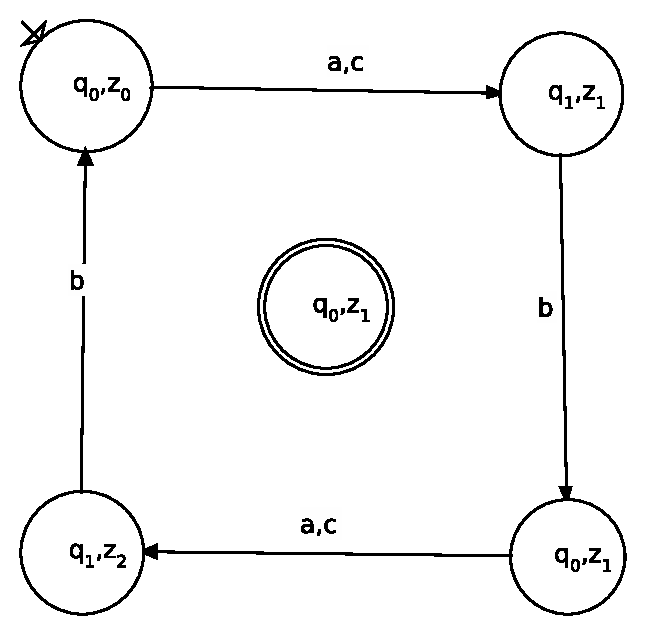
\includegraphics[scale=0.7]{334.pdf}

\subsubsection{}
$L(A_{3}) = \emptyset$\\
$L^\omega(A_{3}) = \emptyset$\\

\subsection{}
\subsubsection{}
Für $TS_1 \leftrightarroweq TS_2$ müsste gelten:\\
$\mathcal{B} = \{(z_0,p_0),(z_2,p_8),(z_1,p_1),(z_2,p_2),(z_0,p_3),(z_1,p_4),(z_2,p_5),(z_0,p_6),(Z2,P4),(z_1,p_7)\}$\\
Da aber $(z_2,p_4)$ nicht in $\mathcal{B}$ liegt, da $z_2$ ein Endzustand ist und $p_4$ nicht sowie von $z_2$ eine c-Kante wegführt und von $p_4$ nur eine b-Kante. Somit sind $TS_1$ und $TS_2$ nicht bisimilar.\\\\
Für $TS_1 \leftrightarroweq TS_3$\\
$\mathcal{B} = \{(z_0,q_0),(z_2,q_1),(z_1,q_2),(z_2,q_3),(z_0,q_4),(z_2,q_5),(z_1,q_6),(z_2,q_7),(z_0,q_8),(z_2,q_9)....\}$\\
Somit sind $TS_1$ und $TS_3$ bisimilar.\\\\
Für $TS_2 \leftrightarroweq TS_3$\\
$\mathcal{B} = \{(p_0,q_0),(p_8,q_1),(p_1,q_2),(p_2,q_3),(p_0,q_4),(p_8,q_5),(p_3,q_4),(p_2,q_5),(p_4,q_6)\\,(p_5,q_7),(p_6,q_8),(p_4,1_9),(p_7...)...\}$\\
Somit sind $TS_2$ und $TS_3$ bisimilar.\\\\
\subsubsection{}
a.) $\mathcal{B}_1 = \{(z_0,q_0),(z_2,q_1),(z_3,q_1),(z_4,q_4),(z_1,q_2),(z_1,q_3)\}$\\
$\mathcal{B}_2 = \{(q_0,z_0),(q_1,z_2),(q_1,z_3),(q_4,z_4),(q_2,z_1),(q_3,z_1)\}$\\
Die Bisimulationsrelation ist eine Menge von Paaren, die für jeden Zustand eine $TS_1$ angibt, welchem Zustand er aus einem $TS_2$ zugeordnet werden kann. Daraus folgt $TS_1 \leftrightarroweq TS_2$. Dadurch ist es nicht relevant in welcher Reihenfolge die Zustände in den Paaren zugeordnet werden. Also gilt $\mathcal{B}_1 = \mathcal{B}_1$ und das bedeutet dass beide die Bedingungen für die Bisimulation erfüllen.\\\\
b.) $\mathcal{B}_3 = (\mathcal{B}_1\cup \mathcal{B}_2)=\{(z_0,q_0),(z_2,q_1),(z_3,q_1),(z_4,q_4),(z_1,q_2),(z_1,q_3)\}\cup \\\{(q_0,z_0),(q_1,z_2),(q_1,z_3),(q_4,z_4),(q_2,z_1),(q_3,z_1)\}$\\
Alle Paare aus der ersten Relation $\mathcal{B}_1$ sind auch in $\mathcal{B}_2$ enthalten. Demnach steht jeder Zustand z aus $TS_1$ in Relation zu einem Zustand q aus $TS_2$ und umgekehrt. Daher erfüllt auch $\mathcal{B}_3$ die Bedingungen für die Bisimulation.\\
c.) Wenn die Kante $(q_1,b,q1)$ entfernt wird, sind $TS_1$ und $TS_3$ nicht bisimilar, da in der Relation das Paar $(z_2,q_1)$ enthalten wäre aber nur von dem Zustand $z_2$ eine b-Kante wegführt. Bei $q_1$ wurde diese Kante entfernt und somit haben $z_2$ und $q_1$ nicht die gleichen Zustandsfolgen und es kann keine Bisimulationsrelation zwischen den beiden TS aufgestellt werden.

\end{document}
